% =============================================================================
% Engineering report -- SC-TPU + RV32I SoC on the Sipeed Tang Nano 9K (rev C).
% Task DOC-02, author of this file: documentation-engineer.
% Input revision: git fab802e (branch claude/awesome-lovelace-hu02o8); HEAD moved
% to 99ee941 during the task (changes only management/EXECUTION_METRICS.md and
% scripts/make_release.sh, no evidence file).
%
% Build:  cd reports/engineering && latexmk -pdf -interaction=nonstopmode \
%                                            -halt-on-error main.tex
% Inputs: status_matrix.tex (stub until gate G4), figures from
%         reports/figures/article_figures.py (log logs/doc/article_figures_revC.log).
%
% Number policy: every number carries a "% evidence: <path>" comment next to
% it and a label in the text or table caption: SOURCE, CALCULATION,
% SIMULATION (golden model, RTL simulation, synthesis / P&R / STA tool
% estimates), ASSUMPTION. No MEASUREMENT exists: no hardware was operated.
% Status words: PASS / PARTIAL / FAIL / BLOCKED / NOT RUN only.
%
% REVIEW HOOK: section "Review findings" (label sec:review) is a placeholder
% until the manager forwards the REV-01 findings
% (reports/review/REVIEW_A_cpu_soc.md, reports/review/REVIEW_B_tpu_model_article.md).
% =============================================================================
\documentclass[10pt,a4paper]{article}

\usepackage[T1]{fontenc}
\usepackage{lmodern}
\usepackage[margin=2.2cm]{geometry}
\usepackage{amsmath,amssymb}
\usepackage{graphicx}
\usepackage{booktabs}
\usepackage{tabularx}
\usepackage{longtable}
\usepackage{array}
\usepackage{xcolor}
\usepackage{enumitem}
\usepackage{url}
\usepackage[hidelinks]{hyperref}

\graphicspath{{../figures/}}
\setlist{itemsep=1pt,topsep=3pt}
\setlength{\emergencystretch}{3em}  % avoid overfull lines with long paths
\newcolumntype{L}{>{\raggedright\arraybackslash}X}
\newcolumntype{P}[1]{>{\raggedright\arraybackslash}p{#1}}  % ragged-right fixed column
\newcommand{\lbl}[1]{\textsc{#1}}          % evidence label in running text
\newcommand{\Dp}{D'}                      % post-processed accumulator (spec: Dp)
\newcommand{\st}[1]{\textbf{#1}}            % status word
% File paths: url-style, breakable at / _ . - so long paths do not overflow.
\def\UrlBreaks{\do\/\do\_\do\.\do\-\do\{\do\,}
\urlstyle{tt}
\DeclareRobustCommand{\file}{\path}   % robust: usable in captions
\renewcommand{\arraystretch}{1.12}

\title{SC-TPU + RV32I SoC on the Tang Nano 9K\\[3pt]
\large Engineering Report --- design revision C}
\author{Author Name (placeholder)\\documentation-engineer, task DOC-02}
\date{2026-11-04 \quad$\cdot$\quad input revision \texttt{fab802e}}

\begin{document}
\maketitle

\begin{center}
\fbox{\parbox{0.92\linewidth}{\small\textbf{Evidence status.} Every result in
this report is \lbl{simulation} (Python golden model, RTL simulation with
Icarus Verilog, or synthesis / place-and-route / static-timing estimates of
the open-source flow), \lbl{calculation}, \lbl{source} or
\lbl{assumption}. \textbf{No hardware measurement exists.} A bitstream was
generated as a proof of routability and was \textbf{never programmed} into a
device. Simulation is not test; passing synthesis and place-and-route is not
hardware validation. Section~\ref{sec:pvp} plans the physical validation that
remains to be done.}}
\end{center}

\tableofcontents

% =============================================================================
\section{Scope, conventions and summary}
\label{sec:summary}

\subsection{System}
The project delivers a system-on-chip for the Sipeed Tang Nano 9K board
(Gowin GW1NR-LV9QN88PC6/\allowbreak I5): a multi-cycle RV32I CPU, 4\,KiB of RAM, a
peripheral block (6 LEDs, UART transmitter, cycle counter, test mailbox) and a
stochastic-computing tensor processing unit (SC-TPU) that runs a 64-16-10
multilayer perceptron for the 8$\times$8 handwritten-digits set. The SC-TPU is
a 16$\times$8 weight-stationary tile of bipolar XNOR multipliers with
accumulative parallel counters (APC), driven by 8-step leap-forward LFSRs.
Its behaviour is specified bit-exactly so that a Python golden model and the
RTL agree bit for bit. There is no firmware: CPU programs are testbench
stimuli generated by a Python assembler.
% evidence: management/PROJECT_DEFINITION.md; design/architecture/ARCHITECTURE.md sec. 1-8, 12; requirements/REQUIREMENTS.md REQ-SYS-015

\subsection{Conventions}
\begin{itemize}
\item Number labels: \lbl{source} (data sheet, standard, paper; listed in
  \file{management/SOURCES.md}), \lbl{calculation} (formula and inputs shown),
  \lbl{simulation} (tool, version, log path), \lbl{assumption} (reason given).
  \lbl{measurement} is reserved for real hardware and does not occur.
\item Status words: \st{PASS}, \st{PARTIAL}, \st{FAIL}, \st{BLOCKED},
  \st{NOT RUN}. Requirement verification statuses are assigned only in the
  status matrix after the independent review (gate G4); this report does not
  pre-empt them.
\item Every number in the \LaTeX{} source has a \texttt{\% evidence:} comment
  with the file it was taken from. Paths are relative to the repository root.
\item Design revisions: rev~A (first frozen spec), rev~B (seed change,
  superseded, negative result), rev~C (current;
  \file{design/architecture/ARCHITECTURE.md} sec.~12,
  \file{management/INTERFACES.json} revision C).
\end{itemize}

\subsection{Key results}
\begin{table}[htbp]
\centering\small
\caption{Headline results of design rev C (all \lbl{simulation} or
\lbl{calculation}; none is a hardware measurement).}
\label{tab:headline}
% evidence: see the per-row comments
\begin{tabularx}{\linewidth}{@{}P{4.4cm}P{4.3cm}P{2.0cm}L@{}}
\toprule
Quantity & Value & Label & Evidence \\
\midrule
SC accuracy, mode 2, $K=8$, deployed seeds & 94.4\,\% (340/360) & \lbl{simulation} & \file{reports/sw/accuracy_revC.json}; Wilson CI 91.6--96.4\,\% \\
Expected-value (EV) and int8 reference & 95.0\,\% (342/360) & \lbl{simulation} & same \\
Seed-ensemble mean, mode 2, $K=8$ (20 offsets) & 92.8 $\pm$ 1.4\,\% & \lbl{simulation} & same \\
RTL vs golden model, rev C & 0 mismatching fields / 1454 inferences & \lbl{simulation} & \file{logs/tpu/sim_tpu_console.log} \\
CPU vs ISS & 176/176 runs (44 programs $\times$ 4 bus timings) & \lbl{simulation} & \file{logs/cpu/sim_cpu_summary.log} \\
SoC end-to-end demo & RESULT 7, LED, UART ``7\textbackslash n'', TOHOST 1 & \lbl{simulation} & \file{logs/soc/tb_soc_demo.log} \\
SoC LUT4 / DFF / BSRAM & 5628 (65\,\%) / 2803 (43\,\%) / 5 (19\,\%) & \lbl{simulation} & \file{reports/fpga/soc/soc_impl.md} \\
SoC Fmax, worst of 3 seeds & 47.46\,MHz (target $\ge29.7$) & \lbl{simulation} & same (STA, not silicon-validated) \\
TPU latency, $K=8$ & 2928 cycles = 108.4\,\textmu s & \lbl{sim.}\,+\,\lbl{calc.} & \file{logs/tpu/tb_sc_tpu_mode2.log} D8 \\
Bitstream & 3\,556\,680 bytes, never programmed & file property & \file{logs/soc/pack.log} \\
\bottomrule
\end{tabularx}
\end{table}
% evidence: reports/sw/accuracy_revC.json (qat_noise sc 2 8: 340/360; EV 342/360; ensemble mean 0.928, sd 0.0143, n 20)
% evidence: logs/tpu/sim_tpu_console.log (474 + 506 + 474 = 1454 golden inferences, 0 mismatching fields, rev C)
% evidence: logs/cpu/sim_cpu_summary.log ("# runs: 176 / 176 PASS"); logs/soc/tb_soc_demo.log (D1..D7 PASS)
% evidence: reports/fpga/soc/soc_impl.md (nwl flow: 5628/8640, 2803/6480, 5/26; Fmax 51.98/47.46/51.21)
% evidence: logs/soc/pack.log (3556680 bytes, sha256 152d3c6d...)

% =============================================================================
\section{Requirements and verification status}
\label{sec:req}

The requirement baseline is \file{requirements/REQUIREMENTS.md} issue~2
(task REQ-02, spec rev C): 82 requirements in eight areas (SYS 17, CPU 10,
TPU 16, AI 11, RES 6, TIM 5, DOC 8, VER 9), each with text, rationale,
source, verification method (A analysis, S simulation, I inspection,
T test on hardware) and acceptance criterion. Method T is never executed in
this project; every T item belongs to the physical validation plan of
Section~\ref{sec:pvp}. Numeric criteria are backed by
\file{requirements/BUDGETS.md} issue~2.
% evidence: requirements/REQUIREMENTS.md (summary table: 82 rows; per-area counts)

\subsection{Status matrix}
% =============================================================================
% status_matrix.tex -- STUB (documentation-engineer, DOC-02).
% The requirement status matrix is produced by the systems-engineer in
% requirements/STATUS_MATRIX.md after the independent review (gate G4,
% task REV-01). Until then no requirement has an assigned verification status
% (requirements/REQUIREMENTS.md, Conventions: all NOT RUN at issue 2).
% Replace this file by the LaTeX rendering of the matrix (one row per
% requirement ID: ID, title, method, status, evidence path, revision).
% =============================================================================
\begin{center}
\fbox{\parbox{0.9\linewidth}{\centering\textbf{Requirement status matrix: pending G4.}\\[2pt]
The matrix (\texttt{requirements/STATUS\_MATRIX.md}) is written by the
systems-engineer after the independent review REV-01. Until then every one of
the 82 requirements keeps the status NOT RUN of
\texttt{requirements/REQUIREMENTS.md} issue 2; the evidence overview in
Table~\ref{tab:evidence-overview} is \emph{not} a verification status.}}
\end{center}


\subsection{Evidence overview (not a status)}
Table~\ref{tab:evidence-overview} lists, for the requirements with numeric
acceptance criteria, the evidence that the specialists reported. It is an
aid for the reviewer and the systems-engineer; the formal status is set in the
matrix above.

{\small
\begin{longtable}{@{}P{1.9cm}P{4.3cm}P{4.9cm}P{3.9cm}@{}}
\caption{Specialist-reported evidence for requirements with numeric acceptance
(\lbl{simulation} / \lbl{calculation}; not a verification status).}
\label{tab:evidence-overview}\\
\toprule
ID & Acceptance (short) & Reported evidence & Evidence file \\
\midrule
\endfirsthead
\toprule
ID & Acceptance (short) & Reported evidence & Evidence file \\
\midrule
\endhead
REQ-SYS-005 & rst latency 2--3 edges; first fetch $\le40$ cycles & 2 edges; first fetch 31 cycles after rst falls & \file{logs/soc/tb_soc_demo.log}, RTL-SOC R1--R5 \\
REQ-SYS-007 & 0 protocol violations; slave $\le4$ cycles (TPU buffer read while BUSY $\le40$, ADR-012) & 0 violations; max 3 cycles in demo; 35 cycles worst TPU stalled read & RTL-SOC, RTL-TPU handoffs \\
REQ-SYS-012 & $|$baud error$|\le2.0$\,\%; 234 clk/bit; frame 2340 & +0.16\,\% (\lbl{calculation}); 234 / 2340 clocks; 0x00 0x55 0xA5 0xFF decoded & \file{logs/soc/tb_soc_bfm.log}, \file{soc_periph.v} \\
REQ-SYS-016 & TOHOST=1 within 200\,000 cycles; RESULT = golden class & cycle 5441; RESULT 7 = golden & \file{logs/soc/tb_soc_demo.log} \\
REQ-CPU-010 & random programs match ISS & 20 random programs $\times$ 4 timings PASS & \file{logs/cpu/sim_cpu_summary.log} \\
REQ-TPU-003 & PARAMS 0x0302\_0810 (mode 2) & 0x03020810 read & \file{logs/tpu/sim_tpu_console.log} D2 \\
REQ-TPU-013 & 0 mismatches vs rev C golden model & 1454 inferences + 239 clamp re-runs, 0 fields & \file{logs/tpu/tb_sc_tpu_mode{0,1,2}.log} \\
REQ-TPU-014 & CYCLES = BUSY edges & = formula $10\cdot2^K+368$, every vector & same \\
REQ-AI-003 & float, EV $\ge94.0$\,\% & 95.0\,\% / 95.0\,\% & \file{reports/sw/accuracy_revC.json} \\
REQ-AI-004 & $\ge90.0$\,\% ($\ge324/360$) at $K=8$ & 94.4\,\% (340/360) & same \\
REQ-AI-005 & $K_{op}\le9$, gap $\le2$\,pp for $K\ge K_{op}$ & $K_{op}=8$, gaps 0.56 / 0.56 / $-0.28$\,pp & same, \texttt{requirement\_checks} \\
REQ-AI-006 & ensemble mean $\ge90$\,\%; $|$deployed$-$mean$|\le2\sigma$ & 92.8\,\%; 1.14\,$\sigma$ & same \\
REQ-RES-001..004 & each resource $\le85$\,\% & worst 65\,\% (LUT4); BSRAM 5/26; DSP 0 & \file{reports/fpga/soc/soc_impl.md} \\
REQ-RES-005 & 10 I/O & 10 & \file{logs/soc/pins.log} \\
REQ-TIM-001 & worst-seed Fmax $\ge29.7$\,MHz & 47.46\,MHz & \file{logs/soc/pnr_nwl_s{1,2,3}.log} \\
REQ-TIM-004 & CYCLES$(K)\le1.10\,N_{budget}(K)$; $K=8$: 3265 & 2928 at $K=8$; all $K$ below bound & \file{requirements/BUDGETS.md} sec.~3 \\
REQ-TIM-005 & CPU-side time reported & only START$\to$RESULT 2948 and reset$\to$TOHOST 5441 (inputs not written by the demo) & \file{logs/soc/tb_soc_demo.log}, ADR-011 \\
REQ-VER-005 & synth, P\&R, pack exit 0 & all exit 0; bitstream sha256 recorded & \file{logs/soc/pack.log} \\
REQ-VER-009 & physical validation plan present & Section~\ref{sec:pvp} (all steps NOT RUN) & this report \\
\bottomrule
\end{longtable}
}
% evidence: management/handoffs/fpga-engineer/RTL-SOC.md (requirements table); management/handoffs/fpga-engineer/RTL-TPU.md; reports/sw/accuracy_revC.json requirement_checks (REQ-AI-005 gap_pp_by_K 8: 0.556, 9: 0.556, 10: -0.278; REQ-AI-006 abs_deviation_over_std 1.137); requirements/BUDGETS.md sec. 3, 7; management/DECISIONS.md ADR-011, ADR-012

% =============================================================================
\section{Architecture and decisions}
\label{sec:arch}

\subsection{Block structure}
\begin{itemize}
\item \textbf{Clock and reset.} One 27\,MHz domain from the board oscillator
  (pin 52), no PLL. Button S1 (assumed pin 3) passes a 2-flip-flop synchroniser
  into a synchronous active-high reset; there is no debouncer.
\item \textbf{CPU} (\file{design/rtl/cpu/}). RV32I multi-cycle FSM (CLEAR,
  FETCH, DECODE, EXECUTE, SHIFT/MEM, WB), register file in two BSRAM blocks
  cleared by a 32-cycle CLEAR state, one 33-bit adder, iterative shifter, no
  CSRs, no interrupts; ECALL, EBREAK, illegal and misaligned events halt the
  core with a trap cause.
\item \textbf{Bus} (\file{design/rtl/soc/soc_bus.v}). Native valid/ready,
  one master; decoder on \texttt{addr[31:28]}; AND-OR read multiplexer;
  unmapped responder (read 0, sticky \texttt{bus\_err}).
\item \textbf{RAM} 4\,KiB BSRAM with byte enables, initialised from the demo
  program; \textbf{peripherals}: LED, UART TX (234 clocks/bit), CYCLE,
  TOHOST.
\item \textbf{SC-TPU} (\file{design/rtl/tpu/}): bus slave and register map
  (\file{sc_tpu.v}), controller FSM (IDLE, LOAD, STREAM, POST)
  (\file{sc_tpu_ctrl.v}), RNG modes (\file{sc_rng.v}), 8-step LFSRs with
  look-ahead register (\file{sc_lfsr8.v}), lane array with 8 input SNGs,
  128 weight SNGs, XNOR, popcount and 16 17-bit APC accumulators
  (\file{sc_lane_array.v}), two-stage post-processing with a 34-bit exact
  shifter (\file{sc_postproc.v}); weight RAM 1 BSRAM, INPUT/BIAS in LUT-RAM.
\end{itemize}
% evidence: design/architecture/ARCHITECTURE.md sec. 1-7; management/handoffs/fpga-engineer/RTL-CPU.md, RTL-TPU.md, RTL-SOC.md (outputs, design summary)

\subsection{Algorithm of one inference}
For layer 1 (64 inputs, 8 tiles) and layer 2 (16 inputs, 2 tiles): clear the
accumulators; per tile load 128 weights and 8 input codes, then run $L=2^K$
stream cycles, each adding $\sum_i \overline{[r_x<x_i]\oplus[r_w<W_{ji}]}$ to
$\mathit{acc}_j$; post-process
$D=2\,\mathit{acc}-N_{in}L$, $B=\lfloor \mathit{bias}\,2^K/128\rfloor$,
$\Dp=D+B$; layer~1 writes HIDDEN $=128+\mathrm{clip}(\lfloor \Dp\,2^{s+7}/2^K\rfloor,0,127)$,
layer~2 writes SCORE $=\Dp$; RESULT is the argmax over lanes 0..9 (ties to
the lowest index). The LFSRs are re-seeded on START and advance only in
stream cycles.
% evidence: design/architecture/ARCHITECTURE.md sec. 5.3 [BIT-EXACT]

\subsection{Architecture decision records}
{\small
\begin{longtable}{@{}P{1.0cm}P{3.2cm}P{6.2cm}P{4.3cm}@{}}
\caption{Summary of the architecture decision records
(\file{management/DECISIONS.md}).}\label{tab:adr}\\
\toprule
ADR & Subject & Decision & Evidence / consequence\\
\midrule
\endfirsthead
\toprule
ADR & Subject & Decision & Evidence / consequence\\
\midrule
\endhead
000 & Specialist execution mode & Specialists first ran as general-purpose subagents obeying their role files; native agent types after a restart (addendum) & process deviation, labelled \\
001 & Accelerator arithmetic & Bipolar SC with XNOR + APC; int8 binary kept as analytical baseline; unipolar SC rejected & first area estimate ($\sim$9 LUT/lane) corrected by ADR-007 \\
002 & Dataflow & 16$\times$8 weight-stationary tile; IL studied as 4/8/16 variant & fully parallel layer needs 8192 FF ($>$6480) \\
003 & RNG decorrelation & Modes 0/1/2 as synthesis parameter, selection by accuracy vs cost & closed by ADR-008/010 (mode 2) \\
004 & CPU micro-architecture & RV32I multi-cycle (most area left for the TPU) & CPI 4.231 at 0 wait states \\
005 & Leap-forward LFSR & 8 steps per stream cycle (8 fresh bits per $r$) & 8 LUT4 and one level per LFSR \\
006 & Spec rev A.1 & Misaligned jump traps on the jump; strict illegal decoding; reset values & applied in CPU/TPU RTL \\
007 & Spec rev A.2, budget corrections & CONFIG clamp read-back, CYCLES definition, reserved offsets, reads while BUSY, BIAS sign extension, widths, margin definition ($\le$85\,\%, $\ge$29.7\,MHz); tile cost 2855 LUT4 / 1454 FF & requirements re-based \\
008 & Rev B & RNG\_MODE 2 default; mode-2 seeds maximally phase-spaced & \textbf{found defective} (ADR-009) \\
009 & Rev B defect; rev C protocol & Translated operand-pair streams; seed rule; pre-registered selection on validation data & SW-02, SW-03 \\
010 & Rev C adopted & C0 = rev A mode-2 seeds; modes 0/1 keep 0xACE1/0xF9DE; R1+R2 documented; PARAMS 0x03 & closes ADR-003/008/009 \\
011 & Requirement adjustments & REQ-SYS-005(b) bound 8 $\to$ 40 cycles; REQ-TIM-005 PARTIAL accepted for V1; release flow \texttt{-nowidelut} & RTL-SOC evidence \\
012 & REQ-02 rulings & TPU buffer reads while loading may take $\le$40 cycles; accuracy thresholds confirmed; vendor-host access remains a user decision & applied by the systems-engineer \\
\bottomrule
\end{longtable}
}
% evidence: management/DECISIONS.md ADR-000..012 and ADR-000 addendum

% =============================================================================
\section{Interfaces}
\label{sec:if}

\subsection{Memory map}
\begin{table}[htbp]
\centering\small
\caption{Memory map (\lbl{source}: ARCHITECTURE.md sec.~4, INTERFACES.json
revision C).}\label{tab:memmap}
% evidence: design/architecture/ARCHITECTURE.md sec. 4; management/INTERFACES.json memory_map
\begin{tabular}{@{}llll@{}}
\toprule
Base & Size & Slave & Notes\\
\midrule
\texttt{0x0000\_0000} & 4\,KiB & RAM (BSRAM) & program + data, reset PC 0; aliased in \texttt{0x0xxx\_xxxx} \\
\texttt{0x1000\_0000} & 0x20 & peripherals & Table~\ref{tab:periph}; offsets 0x14.. read 0 \\
\texttt{0x2000\_0000} & 4\,KiB & SC-TPU & Table~\ref{tab:tpuregs} \\
other & -- & none & read 0, write ignored, \texttt{mem\_ready} returned, sticky \texttt{bus\_err} \\
\bottomrule
\end{tabular}
\end{table}

\subsection{Register maps}
\begin{table}[htbp]
\centering\small
\caption{Peripheral registers, base \texttt{0x1000\_0000} (\lbl{source}).}\label{tab:periph}
% evidence: design/architecture/ARCHITECTURE.md sec. 4.1; management/INTERFACES.json periph_regs
\begin{tabular}{@{}llll@{}}
\toprule
Offset & Name & Access & Content\\
\midrule
0x00 & LED & RW & [5:0], 1 = LED lit (pins are active-low, the top inverts)\\
0x04 & UART\_TX & W & [7:0] byte to send; ignored while busy\\
0x08 & UART\_STATUS & R & [0] tx\_busy (whole frame incl.\ stop bit)\\
0x0C & CYCLE & R & free-running 32-bit cycle counter since reset\\
0x10 & TOHOST & RW & testbench mailbox: 1 = pass, other odd value = fail code\\
\bottomrule
\end{tabular}
\end{table}

\begin{table}[htbp]
\centering\small
\caption{SC-TPU registers, base \texttt{0x2000\_0000} (\lbl{source}; rev~C).}\label{tab:tpuregs}
% evidence: design/architecture/ARCHITECTURE.md sec. 5.4, 10, 12; management/INTERFACES.json tpu.regs
\begin{tabularx}{\linewidth}{@{}lllL@{}}
\toprule
Offset & Name & Access & Content\\
\midrule
0x000 & CTRL & W & [0] START (ignored while BUSY)\\
0x004 & STATUS & R & [0] BUSY, [1] DONE (cleared by START)\\
0x008 & CONFIG & RW & [3:0] LOG2\_L (reset 8, clamped to 4..10, reads back the clamped value), [6:4] ACT\_SHIFT (reset 0)\\
0x00C & RESULT & R & [3:0] argmax class\\
0x010 & CYCLES & R & rising edges with BUSY = 1 of the last inference\\
0x014 & PARAMS & R & [7:0] NL = 16, [15:8] IL = 8, [17:16] RNG\_MODE, [31:24] version 0x03; release build reads 0x0302\_0810\\
0x040--0x07F & INPUT[0..63] & RW & one code per byte, 4 per word, little-endian\\
0x080--0x0BF & SCORE[0..15] & R & signed 32-bit per output lane\\
0x0C0--0x0CF & HIDDEN[0..15] & R & one code per byte\\
0x100--0x17F & BIAS[0..31] & RW & [15:0] signed, read back sign-extended; word $16(l-1)+j$\\
0x800--0xFFF & WEIGHT RAM & RW & 2\,KiB; byte address $\mathit{base}_l+(\lfloor i/8\rfloor\cdot16+j)\cdot8+(i \bmod 8)$, $\mathit{base}_1=0$, $\mathit{base}_2=1024$\\
other & reserved & -- & read 0, writes ignored\\
\bottomrule
\end{tabularx}
\end{table}
Writes to buffers, weights, CONFIG or CTRL while BUSY are ignored; reads
while BUSY return the current storage contents and may be stalled while the
controller owns the memory ports.
% evidence: design/architecture/ARCHITECTURE.md sec. 5.4, 10

\subsection{Bus protocol}
The master holds \texttt{mem\_valid}, \texttt{mem\_addr} (32), \texttt{mem\_wdata}
(32), \texttt{mem\_wstrb} (4; 0000 = read) and \texttt{mem\_instr} stable until
the slave asserts a one-cycle \texttt{mem\_ready}; \texttt{mem\_rdata} is valid in
that cycle; slaves never assert \texttt{mem\_ready} without \texttt{mem\_valid};
little-endian byte lanes. Implemented latencies (\lbl{simulation}): RAM,
peripherals and the unmapped responder answer in the 2nd cycle, the TPU in the
3rd; a TPU read of INPUT/BIAS/WEIGHT during a tile load or post-processing
waits up to 35 cycles (ADR-012 bound 40). There is no bus timeout.
% evidence: design/architecture/ARCHITECTURE.md sec. 3; management/handoffs/fpga-engineer/RTL-SOC.md, RTL-TPU.md (latencies); management/DECISIONS.md ADR-012

\subsection{Top-level ports and pins}
\begin{table}[htbp]
\centering\small
\caption{Top-level ports of \texttt{soc\_top} and their placement in the routed
design (\lbl{source}: CST with cited sources; \lbl{simulation}: P\&R pin
report).}\label{tab:pins}
% evidence: management/INTERFACES.json top_ports; design/constraints/tangnano9k.cst (header sources [A], [B]); logs/soc/pins.log; reports/fpga/soc/soc_impl.md (pin table)
\begin{tabular}{@{}lllll@{}}
\toprule
Port & Dir & Package pin & IO standard & Note\\
\midrule
\texttt{clk} & in & 52 & LVCMOS33 & 27\,MHz oscillator\\
\texttt{btn\_rst\_n} & in & 3 & LVCMOS18, pull-up & S1 = pin 3 is an \lbl{assumption}\\
\texttt{led\_n[0..5]} & out & 10, 11, 13, 14, 15, 16 & LVCMOS18 & active-low LEDs\\
\texttt{uart\_tx} & out & 17 & LVCMOS33 & to the on-board USB-UART bridge\\
\texttt{uart\_rx} & in & 18 & LVCMOS33 & unused (kept)\\
\bottomrule
\end{tabular}
\end{table}

% =============================================================================
\section{Analyses and their assumptions}
\label{sec:analyses}

\subsection{Resource budget versus result}
The pre-RTL budget (\file{requirements/BUDGETS.md} sec.~1) was built
bottom-up on a calibration bench of one 16$\times$8 tile (2855 LUT4 / 1454 FF
in modes 0/1, 2967 / 1678 in mode 2, \lbl{simulation} of P\&R). It predicted
5735 LUT4 (66.4\,\%) and 2489 FF for the rev~A baseline (mode 1).
Table~\ref{tab:budget} compares it with the release build.
% evidence: requirements/BUDGETS.md sec. 0, 1.2, 1.4

\begin{table}[htbp]
\centering\small
\caption{Budget (\lbl{calculation}) versus achieved (\lbl{simulation}).}\label{tab:budget}
% evidence: requirements/BUDGETS.md sec. 0 (summary table)
\begin{tabularx}{\linewidth}{@{}P{3.6cm}P{2.2cm}rP{1.9cm}L@{}}
\toprule
Item & Budget & Achieved & Deviation & Explanation\\
\midrule
SoC LUT4 & 5735 & 5628 & $-1.9$\,\% & right by compensation: TPU $+20$\,\%, CPU $-51$\,\%\\
SoC LUT4 (budget re-evaluated for mode 2 + BSRAM regfile) & 5591 & 5628 & $+0.7$\,\% & deltas of BUDGETS 1.5 applied\\
SoC DFF & 2489 (2713 mode 2) & 2803 & $+12.6$ / $+3.3$\,\% & mode 2 chosen after the budget (+224 FF)\\
SoC BSRAM & 3 & 5 & +2 blocks & CPU register file in BSRAM (option taken)\\
RAM16SDP4 & 56 & 16 & $-33$\,\% & SCORE kept in flip-flops\\
Worst-seed Fmax & 52.12\,MHz & 47.46\,MHz & $-8.9$\,\% & critical path moved from the SC MAC to the CPU\\
TPU latency & $10\cdot2^K+409$ & $10\cdot2^K+368$ & fixed term $-10.0$\,\% & input load overlapped, argmax folded in\\
\bottomrule
\end{tabularx}
\end{table}
Lesson (risk R-16): block-level budgets were off by $+20$\,\% and $-51$\,\%
and matched in total only by compensation; any future change should be
re-budgeted from per-module synthesis of the RTL, using the achieved cost of
about 14.4 LUT4 per MAC lane rather than the bench value of 22.
% evidence: management/RISKS.md R-16; requirements/BUDGETS.md sec. 1.4 notes

\subsection{Latency}
Budget model (\lbl{calculation} with \lbl{assumption} inputs): $O_{tile}=36$
load cycles per tile, 16+2 post-processing cycles per layer, 10 argmax and 3
start/done cycles $\Rightarrow N(K)=10\cdot2^K+409$. RTL (\lbl{calculation}
from the FSM, confirmed by \lbl{simulation} for every $K$ and vector): load
33 cycles (32 BSRAM words + 1; input words read in parallel), 19
post-processing cycles per layer, argmax on the fly, CYCLES counts BUSY edges
only $\Rightarrow \mathrm{CYCLES}(K)=10(2^K+33)+2\cdot19=10\cdot2^K+368$.
REQ-TIM-004 allows $1.10\,N(K)$ (3265 at $K=8$); the margin at $K=8$ is 337
cycles.
% evidence: requirements/BUDGETS.md sec. 3; design/rtl/tpu/sc_tpu_ctrl.v header; logs/tpu/tb_sc_tpu_mode2.log (D8)

\begin{table}[htbp]
\centering\small
\caption{Latency per inference at 27\,MHz: budget (\lbl{calculation}) and RTL
(\lbl{simulation}; time and rate are \lbl{calculation} from the cycle
count).}\label{tab:latency}
% evidence: requirements/BUDGETS.md sec. 3 (table incl. achieved columns), sec. 4
\begin{tabular}{@{}rrrrrrr@{}}
\toprule
$K$ & $L$ & budget $N(K)$ & RTL CYCLES & time [\textmu s] & inferences/s & bound $1.1N$\\
\midrule
4 & 16 & 569 & 528 & 19.56 & 51\,136 & 625\\
5 & 32 & 729 & 688 & 25.48 & 39\,244 & 801\\
6 & 64 & 1049 & 1008 & 37.33 & 26\,786 & 1153\\
7 & 128 & 1689 & 1648 & 61.04 & 16\,383 & 1857\\
8 & 256 & 2969 & 2928 & 108.44 & 9\,221 & 3265\\
9 & 512 & 5529 & 5488 & 203.26 & 4\,920 & 6081\\
10 & 1024 & 10649 & 10608 & 392.89 & 2\,545 & 11713\\
\bottomrule
\end{tabular}
\end{table}
CPU side (\lbl{simulation}, \file{logs/soc/tb_soc_demo.log}): START store to
RESULT load 2948 cycles (CYCLES + 20); reset release to TOHOST 5441 cycles
(201.5\,\textmu s), 981 instructions, CPI 5.51. The demo does not write the 64
input codes (they come from \file{input.hex}), so the CPU-side input-load time
of REQ-TIM-005 was not simulated (accepted for V1, ADR-011). Double-buffered
weight registers would save 9.7\,\% at $K=8$ for +1024 FF
(\lbl{calculation}, not implemented).
% evidence: logs/soc/tb_soc_demo.log (INFO lines); requirements/BUDGETS.md sec. 3 (CPI 5.51 = (5441-31)/981; double buffering N(8) = 2681, -9.7 %)

\subsection{Timing}
The timing budget assumed the SC MAC path (LFSR $\to$ comparator $\to$
popcount $\to$ accumulator) to be critical at 52.12\,MHz and set a rule of at
most 7 LUT levels between registers. In the release SoC the critical path is
in the CPU (21.07\,ns: 8.83\,ns logic, 12.24\,ns routing; instruction register
$\to$ decoder/FSM next state $\to$ ALU operand select $\to$ 32-bit carry chain
$\to$ PC), 92\,\% longer than the PicoRV32 proxy used in the budget; the TPU
alone reaches 60.43\,MHz. The slack against the 33.67\,ns budget period is
12.6\,ns. The nextpnr Gowin timing model is reverse-engineered and not
validated against silicon (risk R-05); this is why the 10\,\% margin exists.
% evidence: requirements/BUDGETS.md sec. 5 (P1, P3, SoC rows); reports/fpga/soc/critical_path_nwl.txt; reports/fpga/tpu/variants.md (il8_m2_nwl 60.43 MHz)

\subsection{Power (estimate only)}
No open-source power model exists for GW1N and the vendor estimator is
excluded by the open-toolchain requirement. The order-of-magnitude estimate
$P_{dyn}=\sum\alpha CV^2f$ with $V=1.2$\,V and $f=27$\,MHz and the achieved
cell counts gives logic 1.1--13.1\,mW, clock tree 1.1--5.4\,mW, BSRAM
2.5--10\,mW and static power of a few to about 20\,mW, i.e.\ about
5--50\,mW for the FPGA core (\lbl{assumption}: activity and capacitance
coefficients and the core voltage are not sourced). Board-level power is
dominated by the USB bridge, regulators and LEDs and is not estimated. No
power value is presented as \lbl{simulation} or \lbl{measurement}.
% evidence: requirements/BUDGETS.md sec. 6 (issue-2 column); requirements/REQUIREMENTS.md REQ-SYS-017

\subsection{UART divider}
$27\times10^6/115200=234.375$; the divider 234 gives 115\,384.6\,Bd, an error
of $+0.16$\,\% in rate ($-0.16$\,\% in bit time), well inside the 2\,\%
tolerance (\lbl{calculation}); the SoC testbench confirms 234 clocks per bit
and 2340 per frame (\lbl{simulation}).
% evidence: requirements/BUDGETS.md sec. 7; logs/smoke/sys_uart.log; management/handoffs/fpga-engineer/RTL-SOC.md (U1/T9)

\subsection{Accuracy study}
\textbf{Set-up.} Bit-exact golden model, 360-image stratified test split
(seed 0), weights \texttt{qat\_noise} with $s=0$ (selected on the 288-image
validation split, then re-trained on all 1437 training images; not re-trained
for rev B or C), $K=4..10$, three RNG modes, deployed seeds and a 20-offset
ensemble (all generators advanced by a common random start offset, numpy
seed 0, which preserves the relative lags of the deployed set). Accuracies
carry the correct count $k$ and a 95\,\% Wilson interval; paired comparisons
use the exact McNemar test (\lbl{simulation}).
% evidence: reports/sw/accuracy_revC.json (split, rng_seeds_of_study, selected_variant); reports/sw/revABC_comparison.md header (statistics)

\begin{figure}[htbp]
\centering
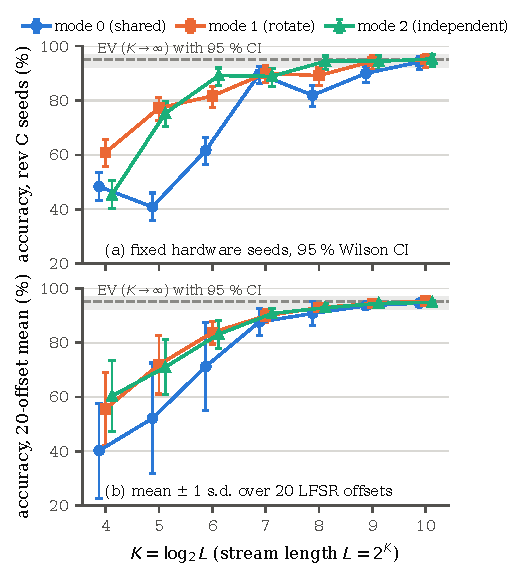
\includegraphics[width=0.48\linewidth]{article_acc_vs_k.pdf}\hfill
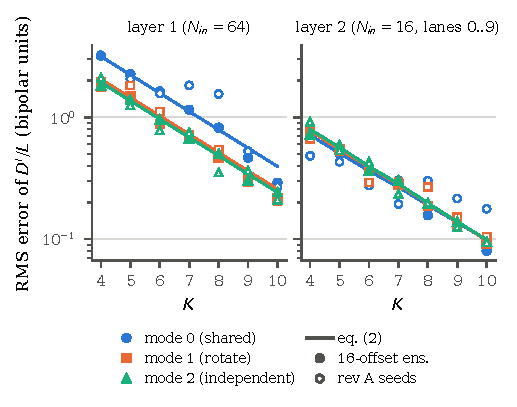
\includegraphics[width=0.48\linewidth]{article_rms_vs_k.pdf}
\caption{Left: test accuracy versus $K$ for the three RNG modes, deployed
rev~C seeds with Wilson CI (top) and 20-offset ensemble mean $\pm$ s.d.\
(bottom). Right: RMS stochastic error of $\Dp/L$ per neuron, ensemble
(filled), eq.~(\ref{eq:var2}) (lines) and deployed seeds (open). All
\lbl{simulation}; data \file{reports/sw/accuracy_revC.json}.}
% evidence: reports/sw/accuracy_revC.json; reports/figures/article_figures.py; logs/doc/article_figures_revC.log
\label{fig:acc}
\end{figure}

\begin{table}[htbp]
\centering\small
\caption{Test accuracy [\%] versus $K$, rev~C (\lbl{simulation}, $n=360$):
deployed seeds ($k$) and ensemble mean $\pm$ s.d.\ over 20 offsets. EV
95.0 (342/360, CI 92.2--96.8). Full CIs in Table II of the article and in the
evidence file.}\label{tab:acc}
% evidence: reports/sw/accuracy_revC.json models.qat_noise.sc, sc_ensemble_accuracy (printed in logs/doc/article_figures_revC.log)
\begin{tabular}{@{}r|rr|rr|rr@{}}
\toprule
$K$ & m0 HW ($k$) & m0 ens. & m1 HW ($k$) & m1 ens. & m2 HW ($k$) & m2 ens.\\
\midrule
4 & 48.3 (174) & 40.2$\pm$17.5 & 60.8 (219) & 55.6$\pm$13.4 & 45.3 (163) & 60.3$\pm$13.1\\
5 & 40.8 (147) & 52.1$\pm$20.4 & 77.2 (278) & 71.8$\pm$10.7 & 75.3 (271) & 71.0$\pm$10.2\\
6 & 61.7 (222) & 71.2$\pm$16.0 & 81.7 (294) & 83.7$\pm$4.2 & 89.2 (321) & 83.0$\pm$5.2\\
7 & 89.7 (323) & 87.5$\pm$4.9 & 90.0 (324) & 89.8$\pm$2.3 & 88.9 (320) & 90.7$\pm$1.7\\
8 & 81.9 (295) & 90.7$\pm$4.4 & 89.2 (321) & 92.8$\pm$1.3 & 94.4 (340) & 92.8$\pm$1.4\\
9 & 90.0 (324) & 93.5$\pm$1.1 & 94.4 (340) & 94.3$\pm$0.8 & 94.4 (340) & 94.4$\pm$0.5\\
10 & 94.2 (339) & 94.5$\pm$0.7 & 95.0 (342) & 95.3$\pm$0.5 & 95.3 (343) & 94.8$\pm$0.5\\
\bottomrule
\end{tabular}
\end{table}

\textbf{Findings.} (1) At $K=8$ the deployed seeds give 81.9/89.2/94.4\,\%
(modes 0/1/2) but the ensemble means are 90.7/92.8/92.8\,\%: a large part of
the spread between modes at one seed set is realisation noise. (2) Mode 0 is
worse in mean and spread (s.d.\ 4.4\,pp at $K=8$) and non-monotonic in $K$.
(3) The mode-1 deployed value at $K=8$ is 2.8 s.d.\ below its ensemble mean,
an unfavourable draw after the rev~B change of the modes 0/1 W seed. (4) The
exact int8 datapath equals the EV model (0 mismatching hidden codes, scores,
results), so EV is the non-SC baseline. (5) Statistical resolution: one image
is 0.28\,pp; Wilson half-widths are 2.3--3.1\,pp between 95 and 90\,\%, so
differences of 1--2\,pp are not resolved.
% evidence: reports/sw/accuracy_revC.json; requirements/BUDGETS.md sec. 8 (mode 1: 2.8 sd below the ensemble mean; CI half-widths)

\subsection{Error model}
With spins $\sigma=2b-1$, uniform cycle-independent $r$ and independent X/W
generators (assumptions A1--A4 of \file{reports/sw/error_model.md}),
\begin{equation}
\mathrm{Var}(\Dp/L)=\frac1L\sum_{\text{tiles}}\Big[\sum_{i,k}C^x_{ik}C^w_{ik}-\Big(\sum_iv_{x,i}v_{w,i}\Big)^2\Big],
\label{eq:var2}
\end{equation}
which reduces to $\frac1L\sum_i(1-v_{x,i}^2v_{w,i}^2)$ for independent lanes
(\lbl{calculation}). Over the rev~C 20-offset ensemble the measured/predicted
RMS ratio is 0.77--1.05 for all 42 layer/$K$/mode combinations
(\lbl{simulation}); mode 2: 0.90--1.05. A single deployed realisation can
deviate by a factor of about 2 (mode 0, layer 2, $K=8$: 0.42 vs 0.19).
Limitations: assumption A2 ignores lagged copies between LFSRs on the common
sequence (rev C minimum 321 stream cycles, X$_0$--W$_3$, coupling only one
operand of two products); the model is per layer and does not propagate
errors through the clipped ReLU. For rev~B, A4 was violated (translated pair
streams) and the model under-predicted mode 2 by 30\,\% and 55\,\% at $K=9$
and 10.
% evidence: reports/sw/error_model.md (derivation, rev B and rev C addenda); reports/sw/accuracy_revC.json error_study (printed in logs/doc/article_figures_revC.log); lfsr_lags

\subsection{Variant studies with identical inputs}
Each variant study changes one factor and keeps everything else identical:
the same trained weights, the same 360 test images and the same 20 offsets
for accuracy; the same synthesis wrapper, constraint file, tool versions,
27\,MHz constraint and placement seeds 1--3 for implementation.
% evidence: reports/fpga/tpu/variants.md (header: wrapper, CST, --freq 27, seeds 1 2 3); reports/sw/accuracy_revC.json (one weight set, one split)

\begin{table}[htbp]
\centering\small
\caption{RNG-mode variants, IL = 8; rule $K$: smallest $K$ within 1\,pp of EV, deployed seeds (implementation: \lbl{simulation} of
synthesis and P\&R of the stand-alone TPU wrapper, rev~A RTL, mode-2 seeds
identical to rev~C; accuracy: \lbl{simulation}, rev~C, $K=8$).}\label{tab:var-rng}
% evidence: reports/fpga/tpu/variants.md (il8_m0/m1/m2 and _nwl rows); reports/sw/accuracy_revC.json (K=8)
\begin{tabular}{@{}lrrrrrr@{}}
\toprule
Mode & LUT4 nwl/def & DFF & Fmax nwl/def [MHz] & HW acc. & ens. mean$\pm$s.d. & rule $K$\\
\midrule
0 shared & 4468 / 4539 & 2445 & 59.44 / 54.95 & 81.9 & 90.7 $\pm$ 4.4 & 10\\
1 rotate & 4461 / 4567 & 2445 & 61.41 / 55.26 & 89.2 & 92.8 $\pm$ 1.3 & 9\\
2 independent & 4572 / 4692 & 2669 & 60.43 / 54.34 & 94.4 & 92.8 $\pm$ 1.4 & 8\\
\bottomrule
\end{tabular}
\end{table}
Mode 2 costs +111 LUT4 (+125 in the default flow) and exactly +224 DFF
(14 extra 16-bit LFSRs) over mode 1; Fmax differences are within seed noise.
Mode 2 was chosen (ADR-008/010) for the smallest stream-length requirement
with the deployed seeds and the smallest seed-to-seed spread at $K=9$; the
ensemble means of modes 1 and 2 at $K=8$ are equal, so the advantage is
modest and rests partly on the deployed realisation.
% evidence: reports/fpga/tpu/variants.md; management/handoffs/fpga-engineer/RTL-TPU.md (RNG_MODE cost); reports/sw/accuracy_revC.json (design_rule, ensemble)

\begin{table}[htbp]
\centering\small
\caption{Input-lane variants, mode 1 (\lbl{simulation}; latency for IL 4/16 is
\lbl{calculation} only, IL = 8 confirmed by simulation).}\label{tab:var-il}
% evidence: reports/fpga/tpu/variants.md (il4_m1, il8_m1, il16_m1 rows, both flows; placement errors)
\begin{tabular}{@{}lrrrrr@{}}
\toprule
IL & LUT4 nwl / def & DFF & Fmax nwl / def [MHz] & CYCLES at $K=8$ & time [\textmu s]\\
\midrule
4 & 3542 / 3693 & 1901 & 65.30 / 71.34 & 5498 & 203.6\\
8 & 4461 / 4567 & 2445 & 61.41 / 55.26 & 2928 & 108.4\\
16 & 6322 / 6699 & 3533 & no legal placement & 1643 & 60.9\\
\bottomrule
\end{tabular}
\end{table}
IL = 16 at 73--77\,\% LUT4 (carry-heavy) failed placement on all attempted
seeds (3 default, 1 \texttt{-nowidelut}; the remaining two were aborted), so
the practical placement limit for such designs can be below the 85\,\% rule.
% evidence: reports/fpga/tpu/variants.md ("Unable to find legal placement", il16_m1_nwl seed 2 aborted, seed 3 not run)

\begin{table}[htbp]
\centering\small
\caption{Training variants (\lbl{simulation}, rev~C seeds, test split; the
selection was made on the validation split).}\label{tab:var-train}
% evidence: reports/sw/accuracy_revC.json models.{float,qat,qat_noise}
\begin{tabular}{@{}llrrrrr@{}}
\toprule
Variant & $s$ & EV ($k$) & mode 2, $K=8$ ($k$) & mode 1, $K=8$ ($k$) & rule $K$ m2 (1\,pp)\\
\midrule
float (post-training rounding) & 1 & 95.3 (343) & 90.8 (327) & 74.7 (269) & none $\le10$\\
qat & 0 & 95.8 (345) & 95.3 (343) & 86.4 (311) & 8\\
qat\_noise (selected) & 0 & 95.0 (342) & 94.4 (340) & 89.2 (321) & 8\\
\bottomrule
\end{tabular}
\end{table}
The differences between qat and qat\_noise on the test split are within one
or two images and not significant; qat\_noise was selected on the validation
split before the test split was used.
% evidence: reports/sw/accuracy_revC.json; management/handoffs/software-engineer/SW-01a.md (selection on validation)

\textbf{Synthesis flow.} On the SoC, \texttt{synth\_gowin -nowidelut} uses 502
fewer LUT4 positions than the default wide-LUT mapping (5628 vs 6130), no
MUX2\_LUT cells (vs 915) and its worst seed is 4.66\,MHz faster (47.46 vs
42.80\,MHz); it is the release flow (ADR-011).
% evidence: reports/fpga/soc/soc_impl.md (flow comparison)

\subsection{\texorpdfstring{Stream length $L=2^K$ as a design rule}{Stream length L = 2\textasciicircum K as a design rule}}
The operating point is the smallest $K$ at which the accuracy stays within a
tolerance of EV for every larger $K$ (Table~\ref{tab:rule}). With the
deployed seeds mode 2 reaches it at $K=8$ for both 1 and 2\,pp; on the
ensemble mean $K=9$. REQ-AI-005 uses the 2\,pp threshold: $K_{op}=8$, with
gaps 0.56, 0.56 and $-0.28$\,pp at $K=8,9,10$. Because 1\,pp is 3.6 images and
below the CI half-width, the rule is an engineering choice, not a statistical
claim. Latency doubles with every step of $K$ (Table~\ref{tab:latency}), so
$K=8$ trades 108\,\textmu s per inference against $\le1$\,pp of accuracy.
% evidence: reports/sw/revABC_comparison.md sec. 4; reports/sw/accuracy_revC.json requirement_checks REQ-AI-005

\begin{table}[htbp]
\centering\small
\caption{Smallest $K$ within 1\,pp $|$ 2\,pp of EV for all larger $K$
(\lbl{simulation}).}\label{tab:rule}
% evidence: reports/sw/revABC_comparison.md sec. 4
\begin{tabular}{@{}llccc@{}}
\toprule
Rev & Basis & mode 0 & mode 1 & mode 2\\
\midrule
A & deployed & 10 $|$ 10 & 9 $|$ 9 & 8 $|$ 8\\
B & deployed & 10 $|$ 10 & 9 $|$ 9 & 10 $|$ 10\\
C & deployed & 10 $|$ 10 & 9 $|$ 9 & 8 $|$ 8\\
C & ensemble mean & 10 $|$ 9 & 9 $|$ 9 & 9 $|$ 9\\
\bottomrule
\end{tabular}
\end{table}

\subsection{\texorpdfstring{Seed-rule study (rev A $\to$ B $\to$ C)}{Seed-rule study (rev A to B to C)}}
\label{sec:seeds}
\textbf{Rev B and its defect.} Rev~B set $X_i=S(4096i)$, $W_i=S(32768+4096i)$
($S(n)$: LFSR state $n$ single steps after \texttt{0xACE1}), maximising the
pairwise phase distance (all 16 generators $\ge512$ stream cycles apart).
Because X and W advance by the same 4096 steps per lane, lane $i$'s
$(r_x,r_w)$ stream is lane $i{-}1$'s delayed by 512 stream cycles, a whole
number of tiles for $K\le9$; identical (tile, lane) count tables recur
(14/54/120/196/100 pairs of 3160 at $K=6..10$, rev~A: 0) and their errors add
coherently. Mode 2 at $K=9$ dropped to 89.7\,\% (323/360) from 94.4\,\%
(340/360): discordant 5/22, exact McNemar $p=0.0015$, difference $+4.7$\,pp
(Newcombe 95\,\% CI $+2.0$ to $+7.8$). At $K=8$ the defect was invisible
(93.9 vs 94.4\,\%, $p=0.79$).
% evidence: reports/sw/revABC_comparison.md sec. 2, 5; reports/sw/error_model.md (rev B addendum); management/DECISIONS.md ADR-009

\begin{figure}[htbp]
\centering
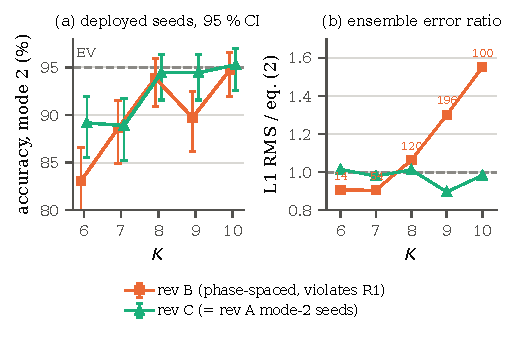
\includegraphics[width=0.55\linewidth]{article_revBC.pdf}
\caption{Mode-2 seed iteration, rev~B versus rev~C (\lbl{simulation}, $n=360$):
(a) deployed-seed accuracy with Wilson CIs; (b) layer-1 ensemble RMS
relative to eq.~(\ref{eq:var2}), with the identical count-table pairs of rev~B.}
% evidence: reports/sw/revABC_comparison.json; reports/figures/article_figures.py
\label{fig:revbc}
\end{figure}

\textbf{Rules.} With $D_i$ the phase offset in single steps between W$_i$ and
X$_i$: \textbf{R1} no two lanes' operand-pair streams are translates
($D_i\ne D_j$, $i\ne j$); \textbf{R2} no direct or swapped shared-bit lag
between operand pairs ($|D_i-D_j|>14$ for $i\ne j$ and $|D_i+D_j|>14$ for all
$i,j$, circular mod 65535; $\pm14$ because $r$ is an 8-bit window of one bit
sequence). R2 is stricter; within the rev~B lattice it is unsatisfiable. Two
independent implementations (software model and budget script) agree: rev~C
satisfies R1 and R2 (minimum pairwise lag 321 stream cycles, next 541), rev~B
violates R1 on 28 of 28 lane pairs and R2 on 28 direct + 36 swapped pairs.
The modes 0/1 pair \texttt{0xACE1}/\texttt{0xF9DE} violates R2 by self-swap
(accepted: non-default study modes, no measured effect; ADR-010 D-B).
% evidence: requirements/REQUIREMENTS.md Conventions (R1/R2); reports/sw/seed_selection_revC.md sec. 1; requirements/BUDGETS.md sec. 9.2 (scripts/budgets/logs/lfsr_rules_revC.log)

\begin{table}[htbp]
\centering\small
\caption{Rev~C seed candidates on the 288 validation images
(\lbl{simulation}; structure \lbl{calculation}). Caveat: these images were in
the final training set; absolute values are optimistic, only the ranking is
used.}\label{tab:cand}
% evidence: reports/sw/seed_selection_revC.md sec. 1, 2
\begin{tabularx}{\linewidth}{@{}lLccrrrr@{}}
\toprule
Cand. & Rule & R1 & R2 & $\lambda_8$ [cyc.] & $K=8/9/10$ ($k$/288) & worst [\%] & rank\\
\midrule
C0 & rev A: $X_i=\texttt{0xACE1}+\texttt{0x3C5A}i$, $W_i=\texttt{0x7A5C}+\texttt{0x2B67}i$ & yes & yes & 321 & 285/285/286 & 98.96 & 1\\
C1 & rev B: $S(4096i)$, $S(32768+4096i)$ & no & no & 512 & 279/274/282 & 95.14 & 5\\
C2 & rev B, W lanes reversed & yes & no & 512 & 276/282/283 & 95.83 & 4\\
C3 & $S(32760i)$, $S(32760(15-i))$ (max $\lambda_8$) & yes & yes & 4095 & 283/284/287 & 98.26 & 2\\
C4 & $S(4095i)$, $S(4095(15-i))$ (max $\lambda_1$) & yes & yes & 3585 & 280/284/285 & 97.22 & 3\\
\bottomrule
\end{tabularx}
\end{table}
\textbf{Protocol and outcome.} The selection rule was fixed before any
accuracy was computed (ADR-009): highest worst-case deployed validation
accuracy over $K\in\{8,9,10\}$, tie-break on the ensemble mean; C3 and C4 were
designed by an exhaustive scan (65\,288 feasible step sizes of 65\,534) from
\lbl{calculation} alone. C0 won by 2 images over C3; among the rule-compliant
candidates no difference is significant (paired McNemar $p\ge0.125$), while
the two rule-violating candidates rank last. Rev~C thus restores the rev~A
mode-2 seeds, now justified by the rules and by held-out data, and keeps the
longest RTL verification history. The test split was evaluated once
afterwards: rev~C equals rev~A in mode 2 image by image (identity asserted
bit-exactly) and rev~B in modes 0/1. Lesson: maximal phase spacing alone is
not a sufficient criterion; the issue-1 risk mitigation that proposed it was
wrong (R-02).
% evidence: reports/sw/seed_selection_revC.md; management/DECISIONS.md ADR-009, ADR-010; reports/sw/revABC_comparison.md (identities); management/RISKS.md R-02

% =============================================================================
\section{Timing and utilisation (three seeds)}
\label{sec:impl}
Flow: Yosys 0.70 (YoWASP) \texttt{synth\_gowin -nowidelut}, nextpnr-0.11.1
himbaechel-gowin, device GW1NR-LV9QN88PC6/I5, family GW1N-9C, CST
\file{design/constraints/tangnano9k.cst}, \texttt{--freq 27},
\texttt{--threads 1}, no \texttt{--timing-allow-fail}; Apicula 0.32
\texttt{gowin\_pack}. All values are tool estimates (\lbl{simulation}).
% evidence: reports/fpga/soc/soc_impl.md (header)

\begin{table}[htbp]
\centering\small
\caption{Release SoC utilisation (identical on all seeds; \lbl{simulation}).}\label{tab:util}
% evidence: reports/fpga/soc/soc_impl.md (nwl table)
\begin{tabular}{@{}lrrrc@{}}
\toprule
Resource & used & device & \% & $\le$85\,\%\\
\midrule
LUT4 (incl.\ ALU and LUT-RAM positions) & 5628 & 8640 & 65 & PASS\\
ALU & 1976 & 6480 & 30 & PASS\\
DFF & 2803 & 6480 & 43 & PASS\\
BSRAM & 5 & 26 & 19 & PASS\\
RAM16SDP4 & 16 & 270 & 5 & PASS\\
IOB & 10 & 276 & 3 & PASS\\
MUX2\_LUT5 / MULT18X18 & 0 / 0 & 4320 / 20 & 0 & PASS\\
\bottomrule
\end{tabular}
\end{table}
(PASS in this table refers to the 85\,\% tool-estimate criterion only; it is
not a requirement status.)

\begin{table}[htbp]
\centering\small
\caption{Post-route Fmax per seed (\lbl{simulation}, static timing of nextpnr;
target $\ge29.7$\,MHz).}\label{tab:fmax}
% evidence: reports/fpga/soc/soc_impl.md; logs/soc/pnr_{nwl,def}_s{1,2,3}.log; logs/cpu/pnr_s{1,2,3}.log; reports/fpga/tpu/variants.md
\begin{tabular}{@{}lrrrrr@{}}
\toprule
Design & seed 1 & seed 2 & seed 3 & worst & margin vs 29.7\,MHz\\
\midrule
SoC, \texttt{-nowidelut} (release) & 51.98 & 47.46 & 51.21 & 47.46 & +59.8\,\%\\
SoC, default flow & 46.47 & 45.79 & 42.80 & 42.80 & +44.1\,\%\\
CPU + RAM alone & 62.46 & 53.26 & 55.74 & 53.26 & +79\,\%\\
TPU alone, IL 8 mode 2, \texttt{-nowidelut} & 64.28 & 64.24 & 60.43 & 60.43 & +103\,\%\\
\bottomrule
\end{tabular}
\end{table}
% evidence (calculation): 42.80/29.7-1 = 44.1 %; 60.43/29.7-1 = 103.5 %
Critical paths (worst seed): SoC 21.07\,ns (CPU instruction register to PC
through the decoder, FSM next state and ALU carry chain); default-flow SoC
23.36\,ns, same path class; TPU alone (\texttt{-nowidelut}) the SC datapath
itself (LFSR or weight register $\to$ comparator carry chain $\to$ XNOR $\to$
popcount $\to$ 17-bit accumulator); TPU alone, default flow (IL 8, mode 1), the 34-bit
post-processing shifter. BSRAM mapping was checked in the routed netlist: 5
blocks, 3 with non-zero initialisation (program RAM, weight RAM), 2 with
all-zero initialisation (register file). All 10 ports sit on their CST pins.
The bitstream (3\,556\,680 bytes, sha256
\texttt{152d3c6d\ldots76258}) is a build product in \file{sim/soc/build/},
regenerated by \file{scripts/synth_soc.sh}.
% evidence: reports/fpga/soc/soc_impl.md (critical path, BSRAM, pins, bitstream); reports/fpga/tpu/il8_m1_critical_path.txt, il8_m1_nwl_critical_path.txt; logs/soc/bsram_init.log; logs/soc/pack.log

% =============================================================================
\section{Verification methodology and results per block}
\label{sec:ver}
All testbenches are self-checking (print \texttt{TEST PASSED} or
\texttt{TEST FAILED}, \texttt{\$fatal} on failure, timeout watchdog) and run
with Icarus Verilog 12.0; RTL lint with Verilator 5.020 \texttt{-Wall}. Each
testbench was also run with an injected fault and had to fail.
% evidence: requirements/REQUIREMENTS.md REQ-VER-001/002/003; management/TOOLCHAIN.md

{\small
\begin{longtable}{@{}P{2.4cm}P{5.6cm}P{3.9cm}P{3.0cm}@{}}
\caption{Verification per block: what was checked and the decisive log line
(\lbl{simulation}).}\label{tab:ver}\\
\toprule
Block / TB & Method and volume & Decisive result & Log\\
\midrule
\endfirsthead
\toprule
Block / TB & Method and volume & Decisive result & Log\\
\midrule
\endhead
Python golden model & two implementations (reference loops / vectorised count tables); 158 unit tests; reference re-generation of every exported vector & \texttt{158 passed}; \texttt{CROSSCHECK TOTAL: 593 vectors x 33 fields, mismatches = 0} & \file{logs/sw/pytest_revC.log}, \file{gen_hex.log} \\
Python test mutation & 11 mutants of the rev C tests (wrong tables, rules, PARAMS, headers, selection) & 11/11 detected & \file{logs/sw/mutation_revC.log} \\
Assembler + ISS & unit tests incl.\ round trip of 48\,502 instruction words & 0 mismatches & \file{logs/sw/pytest_rv32.log} \\
CPU (\file{tb_rv32i_core}) & 44 ISS-checked programs (11 directed, 20 random, 13 trap) $\times$ 4 bus timings; protocol checker P1--P7; signature, trap cause, halt PC, instret, TOHOST, LED, UART compared & \texttt{\# runs: 176 / 176 PASS} & \file{logs/cpu/sim_cpu_summary.log} \\
LFSR unit (\file{tb_sc_lfsr8}) & leap vs 8 single steps, 70\,000 cycles; period; rev C seed tables re-derived (TC7) & \texttt{TC2 LEAP==8x1 70000 cycles, 0 mismatches}; TC7 PASS & \file{logs/tpu/tb_sc_lfsr8.log} \\
Post-processing unit & 53\,328 vectors incl.\ every $K$, $s$, extreme acc/bias & \texttt{mismatches = 0} & \file{logs/tpu/tb_sc_postproc.log} \\
Lane array unit & 9216 stream cycles, forced $r$ at the code boundaries $\times$ all 256 codes & \texttt{TEST PASSED} & \file{logs/tpu/tb_sc_lane_array.log} \\
TPU system (\file{tb_sc_tpu}) & directed D1--D12 (reset values, PARAMS, clamp, read-back, BUSY behaviour, CYCLES, reset during inference, init files); golden vectors per mode: 360 images, 51 corner, 63 sweep (+32 mode-1 $K=4/10$); RNG trace per cycle; protocol checker & 1454 inferences + 239 clamp re-runs, \texttt{mismatching fields 0}; RNG trace 0 mismatches; PARAMS 0x03020810 & \file{logs/tpu/sim_tpu_console.log} \\
SoC system (\file{tb_soc}) & pins-only TB: reset synchroniser, protocol checker, real-time UART receiver and bit-timing checker, demo D1--D7, 44 CPU programs on the SoC & demo D1--D7 PASS (TOHOST cycle 5441, RESULT 7, ``7\textbackslash n''); \texttt{44 / 44 PASS} & \file{logs/soc/tb_soc_demo.log}, \file{cpu_suite_summary.log} \\
SoC fabric (\file{tb_soc_bfm}) & CPU outputs forced: register access, byte lanes, memory-map edges, unmapped access, CYCLE, UART busy & T1--T10 PASS & \file{logs/soc/tb_soc_bfm.log} \\
Lint & 13 TPU configurations, 5 SoC configurations, CPU & \texttt{LINT\_OK}, no warning & \file{logs/tpu/lint_rtl.log}, \file{logs/soc/lint_rtl.log}, \file{logs/cpu/lint.log} \\
\bottomrule
\end{longtable}
}
% evidence: management/handoffs/software-engineer/SW-03.md (checks); SW-01b.md; management/handoffs/fpga-engineer/RTL-CPU.md, RTL-TPU.md, RTL-SOC.md (checks tables); logs listed in the table

\begin{table}[htbp]
\centering\small
\caption{Negative runs (each must end in \texttt{TEST FAILED} with a non-zero
exit; \lbl{simulation}).}\label{tab:neg}
% evidence: logs/tpu/*_inject_fault.log; logs/cpu/neg_sigfault.log, neg_protofault.log; logs/soc/neg_*.log; logs/soc/sim_soc_console.log
\begin{tabularx}{\linewidth}{@{}lLl@{}}
\toprule
Testbench & Injected fault & Result\\
\midrule
\file{tb_sc_lfsr8} & wrong feedback tap in the reference & TEST FAILED\\
\file{tb_sc_postproc} & truncating instead of floor division in the reference & TEST FAILED\\
\file{tb_sc_lane_array} & AND instead of XNOR in the reference & TEST FAILED\\
\file{tb_sc_tpu} & bit 0 of SCORE[0] flipped in the comparison & TEST FAILED (16 mismatching inferences)\\
\file{tb_rv32i_core} & corrupted expected signature; request changed while waiting & TEST FAILED, \texttt{VVP\_EXIT=1} (both)\\
\file{tb_soc} & expected SCORE[0] bit flipped; UART divider 240; \texttt{mem\_ready} without \texttt{mem\_valid} & TEST FAILED (all three)\\
\file{tb_soc_bfm} & LED polarity expected non-inverted & TEST FAILED\\
\bottomrule
\end{tabularx}
\end{table}
These faults target the checkers, references and stimuli; a systematic
mutation campaign of the RTL itself was not run.

\textbf{Not run.} Gate-level (post-synthesis or post-route) simulation:
\st{NOT RUN}, because the flow provides no behavioural models of the Gowin
block RAMs. Hardware test: \st{NOT RUN} (out of scope; Section~\ref{sec:pvp}).
% evidence: reports/fpga/soc/soc_impl.md ("Not done / limits")

% =============================================================================
\section{Review findings}
\label{sec:review}
% REVIEW-FINDINGS-HOOK: replace this section with the findings of
% reports/review/REVIEW_A_cpu_soc.md and reports/review/REVIEW_B_tpu_model_article.md
% (task REV-01), each with severity, disposition and the changed evidence.
\begin{center}
\fbox{\parbox{0.9\linewidth}{\textbf{Pending.} The independent review REV-01
(\file{reports/review/REVIEW_A_cpu_soc.md} for CPU and SoC,
\file{reports/review/REVIEW_B_tpu_model_article.md} for TPU, golden model and
article) was running when this report was written. Its findings, their
severity and their disposition will be summarised here when they are
available. Nothing in this report has been reviewed independently yet.}}
\end{center}

% =============================================================================
\section{Risks}
\label{sec:risks}
{\small
\begin{longtable}{@{}P{0.9cm}P{4.6cm}P{2.8cm}P{6.3cm}@{}}
\caption{Risk register summary (\texttt{management/RISKS.md} issue 2).}\label{tab:risks}\\
\toprule
ID & Risk & State & Note\\
\midrule
\endfirsthead
\toprule
ID & Risk & State & Note\\
\midrule
\endhead
R-01 & SC accuracy too low & MITIGATED & mode 2 K8 94.4\,\%; CI lower bound 1.6\,pp above the 90\,\% threshold \\
R-02 & LFSR correlation / seeds & REALISED (rev B), MITIGATED (rev C) & R1/R2 + pre-registered selection; modes 0/1 pair violates R2 (accepted) \\
R-03 & Resource overflow & RETIRED (frozen design) & 65\,\% LUT4 \\
R-04 & Timing closure & MITIGATED & 47.46\,MHz worst seed \\
R-05 & Open-toolchain maturity & OPEN & no gate-level simulation; timing model and bitstream unvalidated on silicon; IL 16 placement failure below 85\,\% \\
R-06 & Model/RTL bit-exactness drift & MITIGATED (simulation level) & 0 mismatching fields; gate level not run \\
R-07 & Unverifiable data-sheet values & OPEN & vendor hosts blocked; user decision OD-16 \\
R-08 & No hardware validation & OPEN (by scope) & plan in Section~\ref{sec:pvp} \\
R-09 & Pin ambiguity S1/S2 & PARTIAL & S1 = pin 3 still an assumption (PV-05) \\
R-10 & Statistical over-claiming & OPEN & CIs and McNemar used; wording to be checked by the reviewer \\
R-11 & Latency above budget & RETIRED & 2928 $<$ 3265 \\
R-12 & Buffer port sharing & OPEN & stalled read up to 35 cycles (ADR-012 bound 40) \\
R-13 & Repository bloat & MITIGATED & build products ignored \\
R-14 & Optimistic seed selection & OPEN & validation images seen in training; C0 vs C3 not significant \\
R-15 & Revision mix-up A/B/C & OPEN & spec-revision guards in data and scripts \\
R-16 & Budget-method weakness & OPEN & block budgets $+20$\,\% / $-51$\,\% \\
\bottomrule
\end{longtable}
}
% evidence: management/RISKS.md (issue 2)

% =============================================================================
\section{Limitations}
\label{sec:limits}
\begin{itemize}
\item \textbf{Simulation only.} No quantity is a hardware measurement; the
  bitstream was never loaded. Fmax comes from a reverse-engineered,
  not silicon-validated timing model; there are no I/O timing constraints
  (all external interfaces are slow or asynchronous).
\item \textbf{No gate-level simulation} (no behavioural BSRAM models): the
  equivalence of the netlist with the RTL rests on the synthesis tool.
\item \textbf{CPU-side latency incomplete} (REQ-TIM-005 PARTIAL): the demo
  pre-loads the input image; writing 64 codes by the CPU was not simulated.
\item \textbf{Accuracy resolution}: $n=360$; differences below about 3\,pp
  are not significant without paired tests; the seed selection used
  validation images that the final weights had seen.
\item \textbf{Workload}: a 64-16-10 MLP on 8$\times$8 digits; results may not
  transfer to larger networks. The network was not re-trained for rev~B/C.
\item \textbf{Throughput}: $1.09\times10^7$ useful MAC/s at $K=8$ against a
  theoretical $1.08\times10^9$ int8 MAC/s with the hard multipliers
  (\lbl{calculation}; no int8 design built).
\item \textbf{Sources}: Gowin data sheet and memory guide not accessible; BSRAM
  organisation, core voltage and the S1/S2 button-to-pin mapping are
  \lbl{assumption}s.
\item \textbf{No power figure} beyond the order-of-magnitude
  \lbl{assumption}.
\item \textbf{UART RX unused}: a host cannot send data to the SoC in rev~C,
  which limits what a hardware test can do without a design change.
\item \textbf{Single LFSR polynomial}: all generators are lagged copies of one
  sequence; at $K=10$ each generator re-uses its bit sequence shifted by one
  bit after 8192 stream cycles (no measured penalty).
\end{itemize}
% evidence: reports/fpga/soc/soc_impl.md; management/DECISIONS.md ADR-011; reports/sw/seed_selection_revC.md; requirements/BUDGETS.md sec. 4, 6, 9.1; management/SOURCES.md; management/INTERFACES.json (uart_rx unused)

% =============================================================================
\section{Physical validation plan}
\label{sec:pvp}
This plan satisfies the documentation part of REQ-VER-009. \textbf{None of it
was executed in this project}; every step has the status \st{NOT RUN}.
Loading a bitstream into a board is a decision of the user (see the user
manual, \file{reports/engineering/MANUAL.md}). Results obtained by following
this plan are the first \lbl{measurement}s of the project and must be
recorded with instrument, setting, date, board serial and the git revision and
sha256 of the bitstream used.
% evidence: requirements/REQUIREMENTS.md REQ-VER-009; CLAUDE.md (no flashing in the project)

\subsection{Equipment}
\begin{itemize}
\item Sipeed Tang Nano 9K and a USB-C data cable; host PC with
  \texttt{openFPGALoader} (not part of the project tool set) and a serial
  terminal (e.g.\ 115200 8N1, no flow control).
\item USB-UART: the on-board USB bridge of the Tang Nano 9K exposes the FPGA
  UART (pins 17/18) as a serial port (\lbl{source}: CST sources [A]/[B]).
\item Logic analyser ($\ge$4 channels, $\ge$10\,MS/s) or oscilloscope; probe
  access to pin 17 (UART TX), the reset button signal (pin 3) and one LED
  pin.
\item Bench supply (5.0\,V, current limit 0.5\,A) feeding the board through a
  USB-C power breakout, with a current meter (resolution $\le$1\,mA), or an
  in-line USB power meter.
\item Optional: thermal camera.
\end{itemize}
% evidence: design/constraints/tangnano9k.cst (header sources [A], [B]: "Use buildin USB-serial" TXD 17 / RXD 18)

\subsection{Preconditions}
\begin{enumerate}
\item Rebuild the bitstream from a clean checkout of the release revision with
  \file{scripts/synth_soc.sh}; record its sha256 and compare with
  \texttt{152d3c6d\ldots76258} (rev C, \file{logs/soc/pack.log}). A
  different hash after a rebuild is not necessarily an error (record it), but
  then the test result refers to the new file.
\item Re-run \file{scripts/sim_soc.sh} on the same revision and keep the log:
  the hardware result is compared with that simulation.
\item Load the bitstream into the volatile SRAM configuration only (no flash
  write), so a power cycle restores the previous board content.
\end{enumerate}
% evidence: reports/fpga/soc/soc_impl.md (bitstream section); management/handoffs/fpga-engineer/RTL-SOC.md (next actions: scripts)

\subsection{Test items}
{\small
\begin{longtable}{@{}P{1.0cm}P{2.6cm}P{5.4cm}P{4.3cm}P{1.4cm}@{}}
\caption{Physical validation items. Expected values are \lbl{simulation}
results of rev~C unless labelled otherwise; status of every item: NOT RUN.}\label{tab:pvp}\\
\toprule
Item & What & How (equipment, procedure) & Pass criterion & Req.\\
\midrule
\endfirsthead
\toprule
Item & What & How (equipment, procedure) & Pass criterion & Req.\\
\midrule
\endhead
PV-01 & Supply current, unconfigured and configured & Bench supply 5.0\,V via USB-C breakout and current meter (or USB power meter). Record current (a) with the factory/previous configuration, (b) after loading the rev~C bitstream, idle after the demo (the program ends in a loop). Repeat for three power-ups. & Values recorded with the measurement label; no current limit trip; no pass bound exists (REQ-SYS-017 is an estimate: FPGA core 5--50\,mW, \lbl{assumption}, board dominated by the USB bridge). & SYS-017, VER-009(5) \\
PV-02 & 3.3\,V rail (optional) & Multimeter on the 3.3\,V regulator output; the test point must be taken from the official schematic, which was not accessible here (\lbl{assumption}). & Recorded; within the regulator tolerance stated in the schematic/data sheet & VER-009 \\
PV-03 & Configuration (SRAM load) & \texttt{openFPGALoader -b tangnano9k <file>.fs} (see manual); observe the loader's result. & Loader reports success; the design starts (PV-04). & SYS-001, VER-005 \\
PV-04 & LED pattern after reset & Hold the reset button (pin 3), then release; observe the six LEDs. & While held: all six off (\texttt{led\_n}=111111). After release: LEDs on pins 10, 11, 13 lit, 14, 15, 16 off (LED = RESULT = 7; \texttt{led\_n}=111000). & SYS-006, SYS-013, SYS-016 \\
PV-05 & Reset button behaviour and S1/S2 pin assumption & Open the terminal, press and release each button in turn; logic analyser on pin 3 to see bounce. & Exactly one button (expected: silkscreen S1) restarts the demo and the terminal shows a new ``7\textbackslash n''; the other has no effect. Record which label is pin 3; if it is S2, correct the CST comment and SOURCES S-022. Bounce may cause several restarts per press (no debouncer): record their number; repeated ``7'' lines are acceptable. & SYS-005, SYS-014, R-09 \\
PV-06 & UART content & Serial terminal at 115200 8N1 on the board's USB serial port; terminal opened before the reset is released. & Received bytes 0x37 0x0A (``7\textbackslash n'') once per reset; no framing errors. & SYS-012, SYS-016 \\
PV-07 & UART timing / clock & Logic analyser on pin 17 during the transmission; measure the duration of the 10-bit frame of 0x37 and of single bits. & Bit time 8.667\,\textmu s, frame 86.67\,\textmu s (\lbl{calculation}: 234 / 2340 clocks at 27\,MHz); baud within 115200 $\pm$2\,\% (bit time 8.51--8.86\,\textmu s). The measured bit time also gives the oscillator frequency $f=234/t_{bit}$. & SYS-012, SYS-004 \\
PV-08 & Start-up latency & Logic analyser: reset release edge (pin 3) to the falling edge of the first UART start bit. & Compare with the same interval in the SoC simulation (to be extracted from the \file{tb_soc} waveform; not yet extracted). Agreement within a few clock cycles plus the synchroniser latency is expected (deterministic design). & SYS-005, TIM-005 \\
PV-09 & Inference latency (CYCLES) & The demo stores CYCLES at RAM \texttt{0x0E00} but does not transmit it. A future test program (generated with the Python assembler, not firmware) must read CYCLES and CYCLE and send them as hexadecimal text over the UART. & CYCLES = 2928 exactly at $K=8$ (and $10\cdot2^K+368$ for other $K$): the counter is deterministic, so any deviation is a failure. & TPU-014, TIM-004, VER-009(4) \\
PV-10 & RESULT for several images & Requires either (a) $\ge$20 bitstreams with different \file{input.hex}, or (b) a future test program that loops over $\ge$20 images stored in RAM (20 $\times$ 64\,B fits in 4\,KiB) and prints each RESULT. & Each RESULT equals the golden-model RESULT of the same image, mode 2, $K=8$, rev~C (bit-exact expectation: 100\,\% agreement, not an accuracy threshold). & TPU-013, VER-009(3) \\
PV-11 & Accuracy over the test set & Streaming the 360 test images from the host needs a UART receiver in the RTL (unused in rev~C), a test program and a future host script. Not possible with the rev~C bitstream. & Future work: hardware accuracy equals the simulated 94.4\,\% (340/360) image by image. & AI-004 (future) \\
PV-12 & Repeatability & Repeat PV-04, PV-06, PV-07 after three separate power-ups. & Identical results each time. & VER-009(6) \\
PV-13 & Fmax margin by PLL sweep & Future work: a separate test build with a PLL (excluded from rev~C by REQ-SYS-004) sweeping the system clock upward in steps, with the UART divider recomputed per frequency; PV-06/PV-10 at each step. & Correct operation at $\ge29.7$\,MHz; the highest passing frequency is compared with the 47.46\,MHz STA estimate. & TIM-001 (future) \\
PV-14 & Thermal (optional) & Thermal camera on the FPGA package after 10\,min in the demo loop. & Informative only; no hot spot on the board above normal ambient-plus-a-few-kelvin (\lbl{assumption}, no requirement). & -- \\
\bottomrule
\end{longtable}
}
% evidence: logs/soc/tb_soc_demo.log (D4 led_n 111000, D5 "7\n", D6 CYCLES 2928 at 0x0E00); sim/data/soc_demo_prog.lst (program ends in halt_loop; CYCLES stored at 0x0E00, not transmitted); requirements/BUDGETS.md sec. 7 (234 clocks/bit); management/INTERFACES.json (uart_rx unused); management/SOURCES.md S-022 (S1/S2 conflict)
% evidence (calculation): bit time 234/27e6 = 8.667 us; frame 2340/27e6 = 86.67 us; +/-2 % of 115200 Bd = 112896..117504 Bd -> 8.857..8.510 us

\subsection{Order and stop criteria}
Run PV-01 (unconfigured), PV-03, then PV-04 to PV-07, PV-12 and PV-01
(configured); PV-08 to PV-11 and PV-13 need additional work. Stop and
disconnect if the supply current trips the limit, the board heats noticeably
or the loader reports an error. Any failure is recorded as a hardware
\st{FAIL} with the evidence and does not invalidate the simulation results,
which remain labelled as such.

% =============================================================================
\section{Reproduction}
\label{sec:repro}
The commands to reproduce every result, the expected decisive output lines,
the repository map and troubleshooting are in the user manual
\file{reports/engineering/MANUAL.md}. Main entry points:
\file{scripts/sim_cpu.sh} ($\sim$10\,s), \file{scripts/sim_tpu.sh}
($\sim$45\,min), \file{scripts/sim_soc.sh} ($\sim$2\,min),
\file{scripts/synth_soc.sh} ($\sim$45\,min single-threaded), and in
\file{code/python}: \texttt{python -m sctpu.accuracy --spec-rev C
--ensemble-size 20}, \texttt{python -m sctpu.seed\_select},
\texttt{python -m sctpu.compare\_abc}.
% evidence: management/handoffs/fpga-engineer/RTL-SOC.md (next actions: run times); reports/sw/accuracy_revC.json command; reports/sw/seed_selection_revC.md, revABC_comparison.md (commands)

\end{document}
